\documentclass[9pt,conference]{IEEEtran}
\usepackage[nomarkers]{endfloat}
\usepackage[cmex10]{amsmath}
\usepackage{filecontents}
\usepackage{lipsum}
\usepackage{graphicx}

\begin{filecontents*}{informe.bib}
@electronic{refmallba,
  % author        = {Universidad de Málaga},
  title         = {Referencia Mallba/Malva},
  url           = {http://neo.lcc.uma.es/mallba/easy-mallba/index.html},
  % year          = {2008}
}
\end{filecontents*}

\begin{document}

%-------- Metadata -------- 
	\title{Pr\'actico 1}
	\markboth{Algoritmos Evolutivos 2015}{Shell \MakeLowercase{\textit{et al.}}: A Novel Tin Can Link}
	\author{
		\IEEEauthorblockN{Gonzalo Torterolo}
		\IEEEauthorblockA{
			Facultad de ingenier\'ia\\
			UDELAR\\
			Montevideo, Uruguay\\
			Email: gonzalo.torterolo@fing.edu.uy
		}
		\and
		\IEEEauthorblockN{Gisel Cincunegui}
		\IEEEauthorblockA{
			Facultad de ingenier\'ia\\
			UDELAR\\
			Montevideo, Uruguay\\
			Email: gisel.cincunegui@fing.edu.uy
		}
	}



% ------- Contenido -------
	\maketitle

	\begin{abstract}
	En el presente informe el objetivo es probar las ventajas y limitaciones de las actuales librerias que implementan algoritmos gen\'eticos mediante la resoluci\'on de 2 problemas t\'ipicos de computaci\'on. Adem\'as se realizan pequeños analisis de las soluciones con el fin de verter conocimientos te\'oricos adquiridos en el curso.
	\end{abstract}
	\begin{IEEEkeywords}
	Algoritmos Evolutivos, AE, Algoritmos Gen\'eticos, AG, Malva, Mallba, Whatchmaker, Knapshak, Mochila
	\end{IEEEkeywords}

	\section{Introducci\'on}
	En la consigna presentada (ver letra en \cite{refmallba}) se deben resolver dos variantes del problema de la mochila (explicadas en la consigna tambi\'en) utilizando ideas de los algoritmos gen\'eticos.

	Por otra parte, el an\'alisis y modelado del problema as\'i como las ventajas de utilizar este tipo de algorimos para el escenario queda relegado a una segunda instancia, pues ya estaban resueltos en las consignas. En todo momento prim\'o la aplicaci\'on de los conceptos te\'oricos del curso antes que la obtenci\'on de resultados como rendimiento, modularidad, etc. No nos interesa, por lo tanto, seguir aqu\'i un enfoque pr\'actico para esta primer aproximaci\'on a los algoritmos evolutivos donde ambos problemas son t\'ipicos y ampliamente estudiados.


	\subsection{Aplicaci\'on de AG}

	Se analizan las diferentes soluciones a las dos variantes del problema de la mochila aqu\'i presentadas, concluyendo con una implementaci\'on para ambos casos.
	Para comenzar a definir las soluciones a los problemas se debe determinar las siguientes car\'acter\'izticas de importancia para un AE t\'ipico.

	\begin{enumerate}
		\item Codificaci\'on.
		\begin{itemize}
				\item Tratamiento de codificaciones no factibles.
		\end{itemize}
		\item Poblaci\'on inicial.
		\begin{itemize}
				\item  Evaluaci\'on de coste/beneficio de utilizar criterios inteligentes de inicializaci\'on.
				\item  Velocidad de convergencia a un \'optimo.
		\end{itemize}
		\item Funcion de fitness.
		\begin{itemize}
				\item  Car\'acter\'izticas especiales requeridas (e.g.: no negatividad de la funci\'on para selecc\'ion proporcional)
				\item  Transformaci\'on para otros escenarios (e.g.: aplicaci\'on para maximizaci\'on/minimizaci\'on)
				\item  Ajustes para mejorar soluciones (escalado, par\'ametros de configuraci\'on).
		\end{itemize}
		\item Seleccci\'on:
		\begin{itemize}
				\item  Elitismo o no.
		\end{itemize}
		\item Cruzamiento.
		\item Mutaci\'on.
		\item Remplazo.
	\end{enumerate}

	\subsection{Particularidades y observaciones de las implementaci\'on/Librerias}
	\begin{itemize}
		\item Malva
		\begin{itemize}
			\item Malva utiliza otro concepto para la mutaci\'on, la probabilidad se aplica por individuo y no por gen.
			\item Parece bastante desprolija, aunque quiz\'as mucho m\'as performante y escalable que cualquier otra, pero como ya se dijo, estas car\'acter\'izticas no interesan en este momento.
		\end{itemize}

		\item Whatchmaker
		\begin{itemize}	
			\item Permite elitismo y esta cantidad es extra a la de la poblaci\'on especificada.
		\end{itemize}
	\end{itemize}


	\subsection{Problemas de los aperitivos}
	
	Para este primer problema interesa obtener el \'optimo de un problema. La aplicaci\'on de AE no nos parec\'io muy adecuada, pues no se estaba buscando una solución aceptable, sino que solo la mejor solución posible es aceptable para los comensales. Por otra parte, el problema es multimodal y NP computacionalmente dificil, lo que lo hace atractivo a una solución de AG.
	En esta variante del problema de la mochila se buscan soluciones enteras pero se aceptan repeticiones, y no existen pesos, o puede entenderse que el peso es proporcional a la ganancia o costo (es el mismo).
	Se utilizó la libería Malva en este problema.
	Se definen las caracterizticas de la solución relativas al AG:

	Notación
		$$X_i,C_i,O$$\\ son la cantidad de aperitivos, costo de aperitivo para el tipo $i$ y costo objetivo\\

	\begin{enumerate}
		\item Codificaci\'on.
		Nos es importante utilizar una codificación conveniente a para facilitar el trabajo del cruzamiento y utilizar SPX o cruzamiento uniforme que ya se encuentran implementadas.

		\item Evaluamos la posibilidad de utilizar 2 tipos de codificaciones.
			La primera de ella muy parecida a la pedida en el próximo problema, donde asignamos un gen binario (los alelos toman valores en \{0,1\}) para cada posible aperitivo en caso de que se elija o no. En el caso deberíamos asignar una cota a la cantidad del genoma, dada por \ref{eq_tope_rep} para cada tipo de aperitivo. Esta codificación es bastante intuitiva pero tiene la desventaja de asignar varios genotipos a un mismo fenotipo. El cruzamiento SPX tiene un comportamiento menos discruptivo en esta representación. Podría ser útil en etapas avanzadas de la evolución.

			\begin{equation}
			\label{eqn_tope_req}
			M_i = \lceil \frac{N}{C_i} \rceil
			\end{equation}

			Otra codificación elimina el problema de que varios genotipos se correspondan con un mismo fenotipo. La misma consite en una representación de enteros, donde cada gen representa la cantidad de aperitivos de un tipo dado. Aplicada junto a un cruzamiento SPX esta codificación tiene un comportamiento más discruptivo que la anterior, se mueve por bloques.

			Se puede incluso, utilizar ambas representaciones en distintas etapas de la evoluciones, de hecho propondremos una función de fitness que es {compatible} para ambas codificaciones.

			En las codificaciones anteriores se le puede agregar semántica en el ordenamiento del cromosoma. Se discute la posibilidad de ordenar los genes dentro del cromosoma en función del costo.

			Para la implementación se elige la segunda opción, sin agregar información en el ordenamiento.
		
		Todas las soluciones representables serán consideraciones factibles.

	\item Selección
		Usaremos selección proporcional tanto para la selección de cruzamiento como selección generacional, ya implementada en malva utilizando el algoritmos de la ruleta. La función de fitness toma valores positivos, por lo que es adecuada para este tipo de selección.
		proporción de selección
		pj = Fj/Sum(Fi)

	\item Fitness
		Tomaremos como función de fitness la distancia al valor objetivo.
		Podemos configurar la librería Malva para resolver un problema de minimización en vez de maximización, por lo que no hacé falta transformar la función de fitness.
		\[ v = |\sum\limits_{i=0}^{N} (C_i X_i) - O| \]
		es la distancia del valor objetivo.

	\item Cruzamiento
		Se ha enfocado la elección de las anteriores caracterízticas de AG para utilizar SPX, pero otros algoritmos de cruzamientos donde se apliquen operadores numéricos podría surgir, como por ejemplo, se propone el promedio entre valores de cada padre, o diferentes promedios ponderados. Sin embargo, para la implementación se opta por SPX.

	\item Mutación
		Se utilizó una mutación uniforme sobre los valores posibles de alelo de cada gen, expresada por la formula:
		\[ B_i = (B_i + rand(0,M_i)) \% M_i \]


	Población inicial
		La población inicial será muy importante para determinar una buena solución, pues a partir de ella se tiene casi todo el material genético nuevo. En las ejecuciones donde se ha probado la probabilidad de mutación baja hace que no se genere nuevo material genético más del aportado por la población inicial. Sin embargo, una cantidad suficiente de individuos en cada generación logra cubrir el espacio de busqueda bastante bien. Para la generación de la población inicial se utilizó un criterio aleatorio, pero se asegura que existen al menos un aperitivo de cada tipo al asignar el máximo valor factible a en algún gen de cada individuo (el gen numero de individuo \% cantidad de genes del cromosoma).
	\end{enumerate}

	\subsection{Problemas de la mochila}


	\begin{enumerate}
	\item Descripcion del problema:
	El problema es un problema de optimización combinatoria perteneciente a la familia de problemas N-P difíciles. El problema se define de la siguiente manera:
	Dados un conjunto de n objetos, cada uno con una ganancia asociada gi y un peso asociado pi, el objetivo del problema es encontrar el subconjunto de objetos que maximiza la ganancia total, manteniendo el peso total por debajo de la capacidad máxima de la mochila (W).	
	
	\begin{equation}
	\label{eqn_tot_gain}
	x = \sum\limits_{i=0}^{n} g_{i}x_{i}
	\end{equation}

	\begin{equation}
	\label{eqn_tot_peso}
	x = \sum\limits_{i=0}^{n} p_{i}x_{i} < W
	\end{equation}

	
	\item Descripción de la solución:
		Este problema constiste en obtener una solución lo mas próxima posible a la óptima del problema, implementando para ello técnicas de algoritmos evolutivos.
	
		A continuacion se detallará las desiciones para la implementacion del algoritmo evolutivo del problema de la mochila:
	
	\item Codificacion:
		\begin{itemize}	

		\item Arreglo binario con el largo igual a la cantidad de elementos totales que puedo incorporar en la mochila, donde cada posicion del arreglo correspone a el objeto $i$ de la solución. Dicho arreglo será ordenado por peso, manteniendo la referencia del ordenamiento del arreglo original, ya que se busca con esto que la operacion de cruzamiento operada por el algoritmo evolutivo intente probar distintos valores de ganancia ``manteniendo'' relativamente el peso de la solucion mas factible.
		El odenamiento de el arreglo se hará manteniendo dos estructuras de indices para la codificacion (arreglo original -> arreglo ordenado , fenotipo -> genotipo) y la decodificacion (arreglo ordenado -> arreglo original, genotipo -> fenotipo).
		La función de fitness se evaluará con el fenotipo, las operaciones se realizaran con el genotipo, y el resultado retornará el fenotipo de la mejor solucion encontrada.

		\item Factibilidad de la solucion:\\ Se tomará como solucion factible aquella que no sobrepase el limite de peso de la mochila.
		\end{itemize}	
			
	\item Población inicial:\\
		Para la población inicial se optó por la generacion aleatoria de los individuos, pues podemos ver que en varias ejecuciones se alacanza rápidamente un óptimo del problemas.
		
	\item Funcion de fitness:\\
			La ecuacion final de la misma ha mutado de acuerdo a problemas que se nos han planteado a lo largo de la implementacion. Al principio se optó por lo siguiente:	
		\begin{itemize}	
			\item Funcion con penalizacion:\\
			La idea de esta función es mantener los individuos no factibles a lo largo de las generaciones para evitar la deriva genética, ya que los mimos pueden brindar informacion relevante para llegar a la optimizacion de la solucion final.
			Si el peso total del individo no sobrepasa al maxímo permitido para la mochila(candidato factible), la función de fitness retornará la ganancia total del individo evaluado.
			Si el peso sobrepasa el máximo estipulado (candidato no factible), la ganancia total se penalizará restando la ganancia proporcional a la diferencia de peso, quedando a formúla como la siguiente:
				\[ G_{tot}-(frac{2 G_{tot} (k-p)}/k) \]
			\item Funcion sin penalizacion:\\
				Como la solución anterior presentó problemas con respecto a la solucion retornada por el algoritmo, debido a que se devolvian soluciones no factibles, se optó por solo maximizar la ganancia, e implementar otros mecanimos para cuando nos topamos con casos de no factibilidad que se detallará más adelante.
		\end{itemize}	
		
	\item Selección\\
		Para la selección se optó utilizar el mecanismo de la selección proporcional implementada con el algoritmo de la ruleta, para poder mantener individuos menos factibles en la poblacion generacional y así evitar la deriva genetica.
		
	\item Cruzamiento\\
		\begin{itemize}	
		\item SPX. Idema anterior.
		\item Cruzamiento con probabilidad 0.75

		\item Para la selección se optó utilizar el mecanismo de la selección proporcional implementada con el algoritmo de la ruleta, para poder mantener individuos menos factibles en la poblacion generacional y así evitar la deriva genetica.

		\item Para evitar el problema de obtener individuos no factibles, lo que se realizó fue que luego de aplicar la operacion de cruzamiento se evalúa la factibilidad de los mismos, si estos no son factibles se realizará una mutación a el objeto que tenga menos peso, con valor 1 en la codificacion. (otra opcion seria mutar algun objeto aleatoriamente o a aquel que posea menos ganacia), y aplicar esto hasta conseguir la factibilidad del candidato. Asi, logramos no tener candidatos no factibles, y por lo tanto no tener soluciones no factibles. 
		\end{itemize}	
	
	\item Mutación.
		Mutación de bit aleatorio con probabilidad 0.01.
	
	\item Condición de parada:
		10000 generaciones.
	\end{enumerate}

% *Probar variando los parametros (cantidad de población, mutación, escalara la función de fitness, velocidad de convergencia).
% *Explicar pq estamos usando elitismo (remplazo).
% *Hacer un algoritmo de fuerza bruta para hallar mejor solución en casos pequeños.
% 	Para tratar de responder si existe solucion y si hay mas de una.
% *Graficar fitness vs tiempo de ejecucion vs poblacion inicial.
% *Pensar en la distancia del espacio de busqueda.
% 	*Para generar una buena pob inicial.


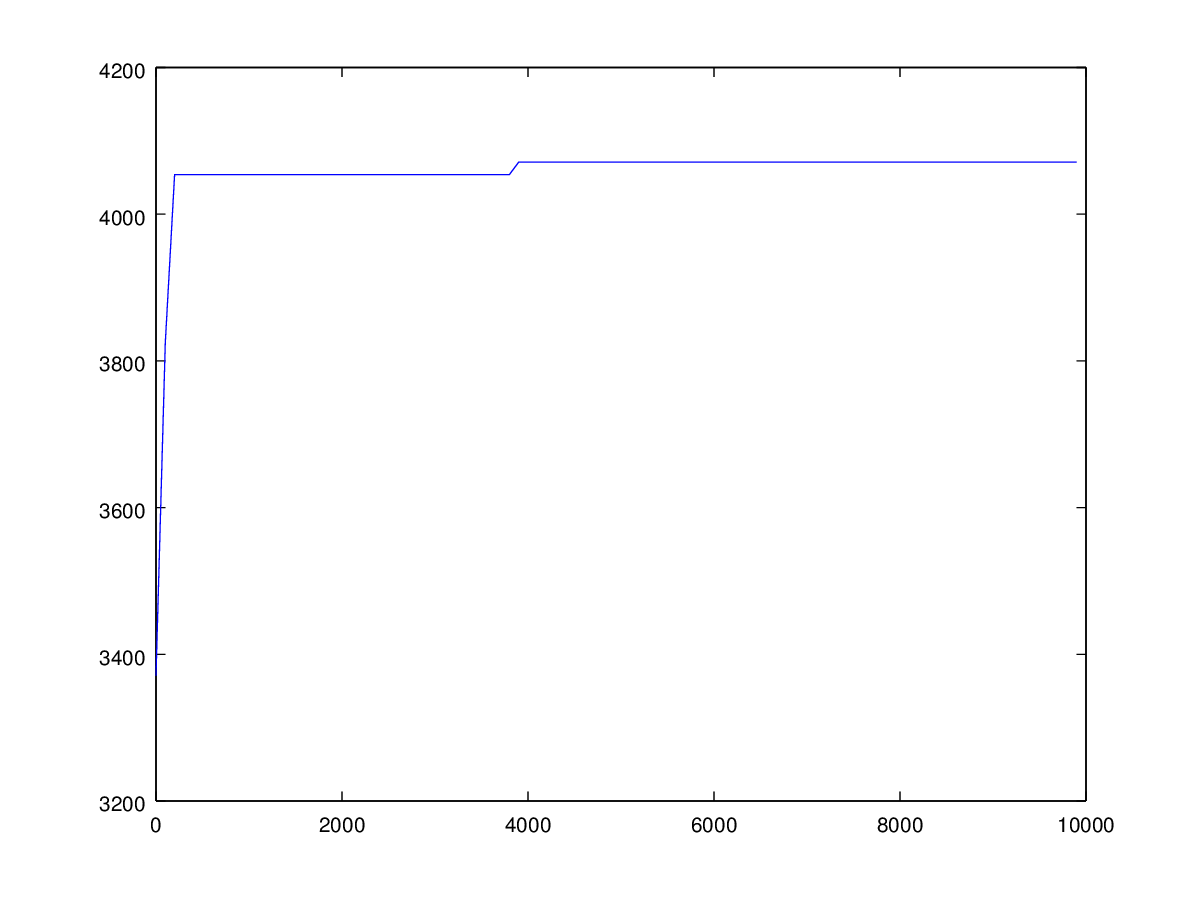
\includegraphics[width=0.5\textwidth]{images/graf_test_in.png}
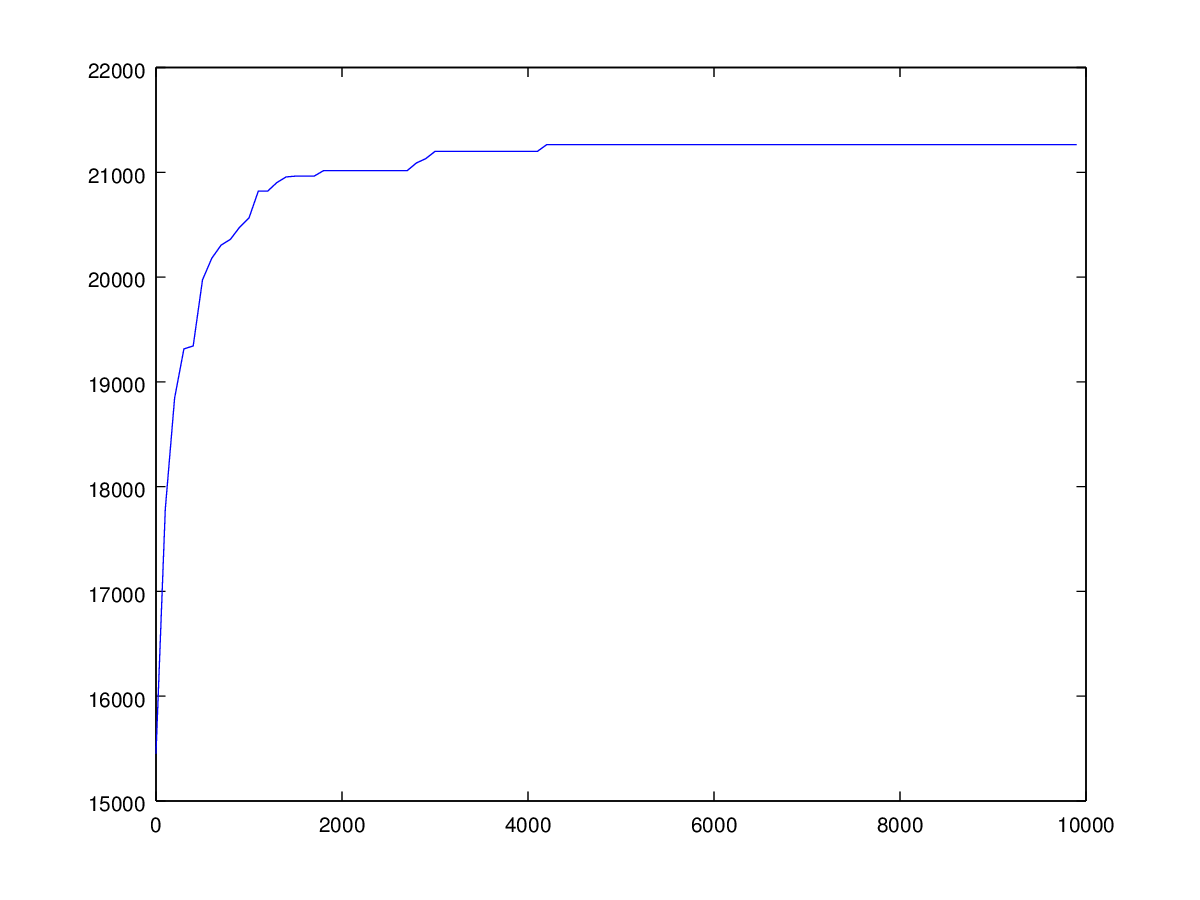
\includegraphics[width=0.5\textwidth]{images/graf_1.png}
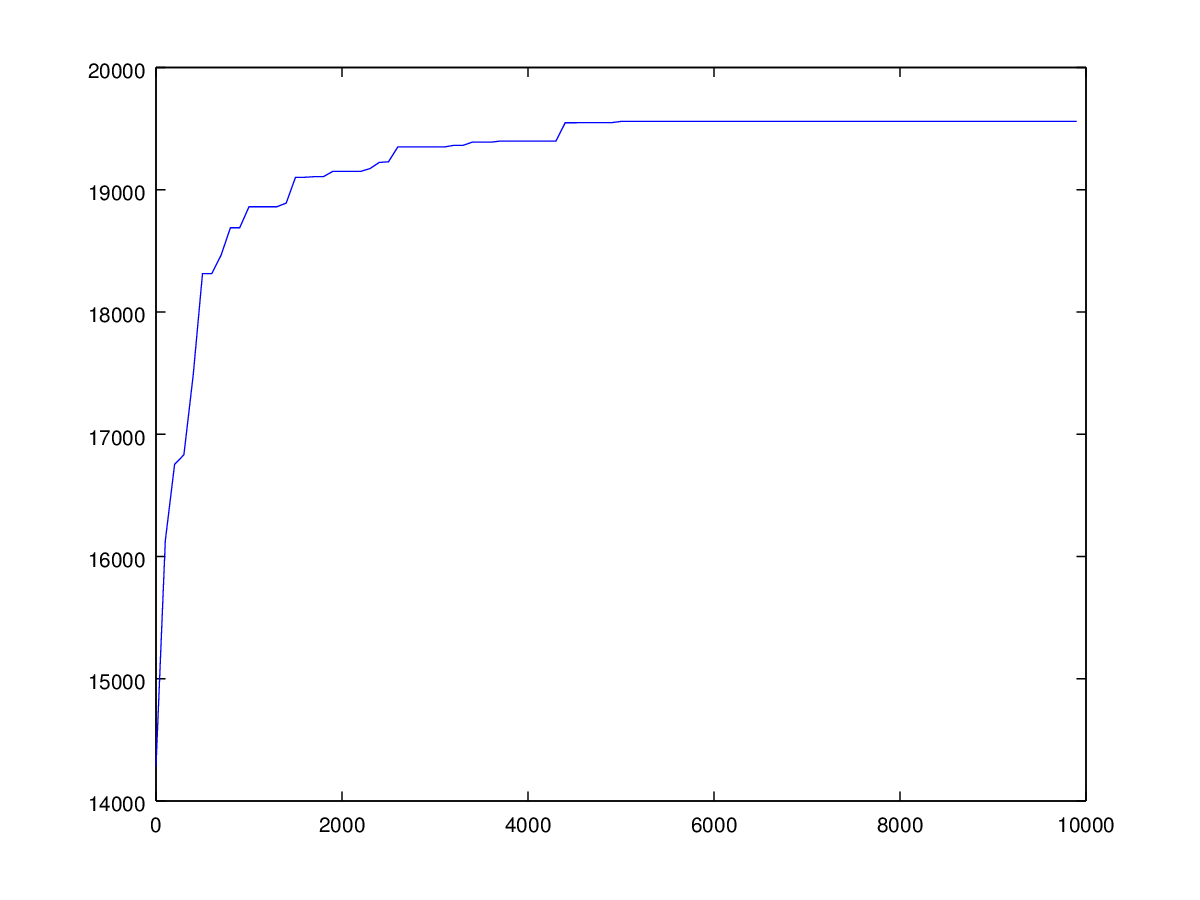
\includegraphics[width=0.5\textwidth]{images/graf_50.png}
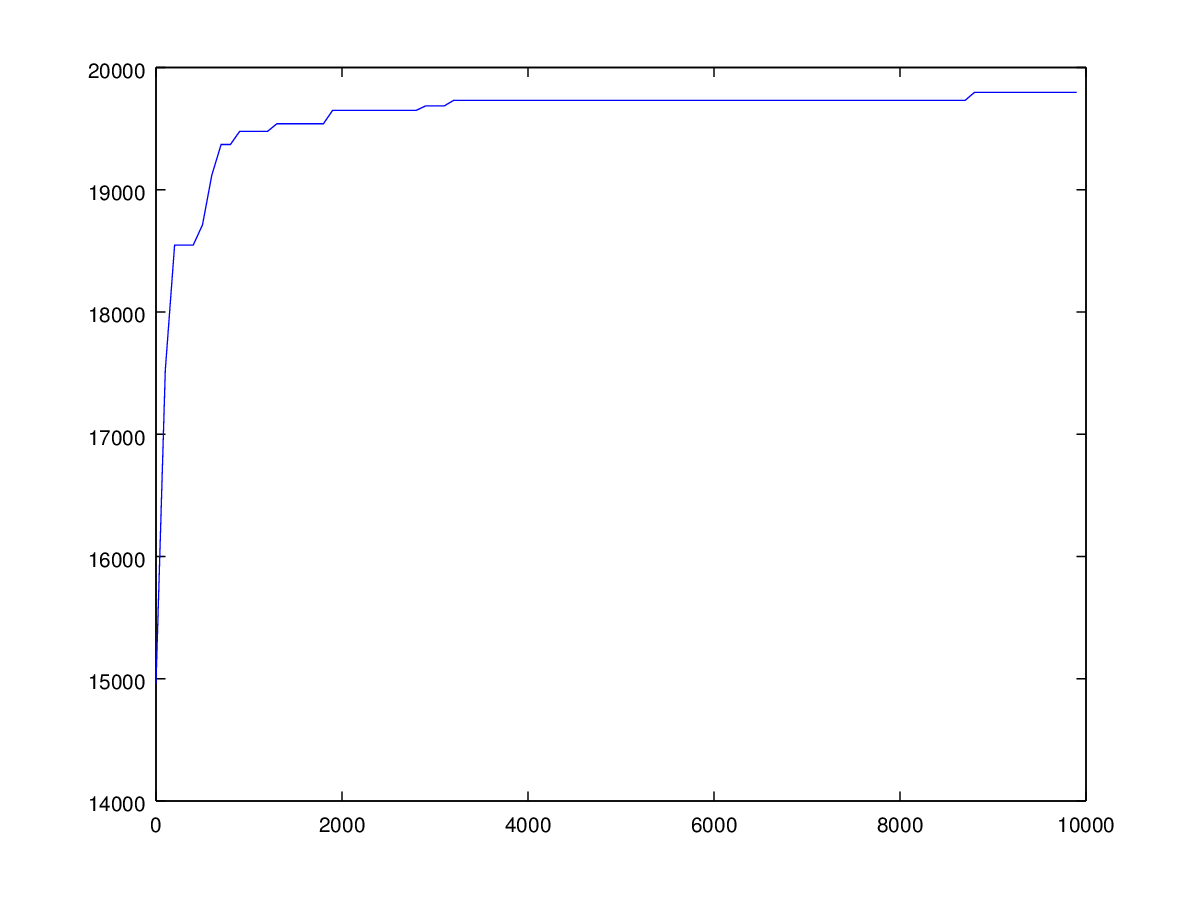
\includegraphics[width=0.5\textwidth]{images/graf_78.png}
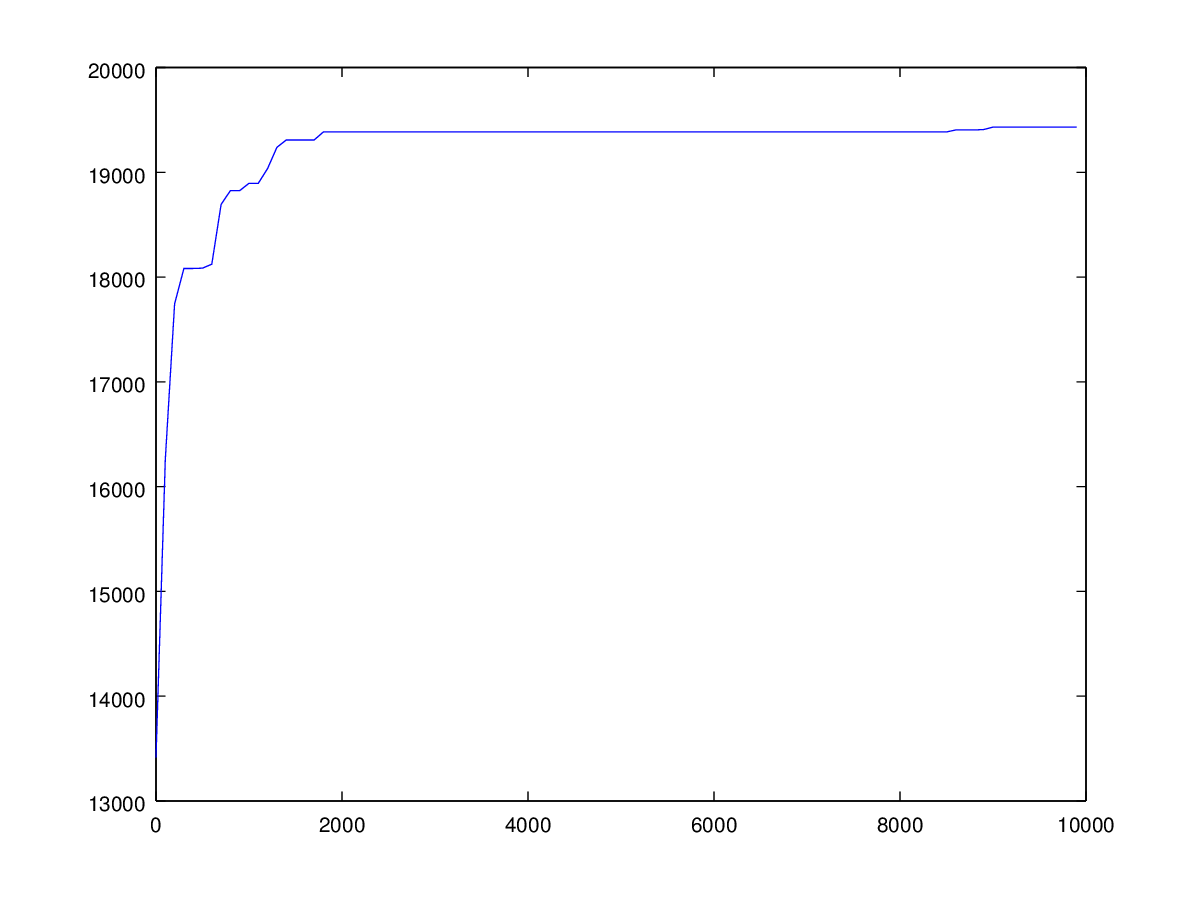
\includegraphics[width=0.5\textwidth]{images/graf_90.png}


\begin{IEEEeqnarray}{rCl}
Z&=&x_1 + x_2 + x_3 + x_4 + x_5 + x_6\IEEEnonumber\\
&&+\:a + b%
\end{IEEEeqnarray}

\begin{IEEEeqnarray}{Rl}
Z=&x_1 + x_2 + x_3 + x_4 + x_5 + x_6\IEEEnonumber\\
&+\:a + b%
\end{IEEEeqnarray}


\begin{IEEEeqnarray}{rCl}
A_1&=&7\IEEEyesnumber\IEEEyessubnumber\\
A_2&=&b+1\IEEEyessubnumber\\
\noalign{\noindent and\vspace{\jot}}A_3&=&d+2\IEEEyessubnumber%
\end{IEEEeqnarray}


\begin{IEEEeqnarray}[\setlength{\nulldelimiterspace}{0pt}]{rl,s}&x,&for $x \geq 0$\IEEEyesnumber\IEEEyessubnumber\\*
[-0.625\normalbaselineskip]
\smash{|x|=\left\{\IEEEstrut[3\jot][3\jot]\right.}&&
\nonumber\\*[-0.625\normalbaselineskip]
&-x,&for $x < 0$\IEEEyessubnumber
\end{IEEEeqnarray}


% Puntos a tocar en el informe:
% 	Para el ejercicio 1:
% 		¿C\'ual fue la soluci\'on encontrada?
% 		¿Se encontr\'o m\'as de	una soluci\'on?
% 	Para el ejercicio 2:
% 		¿Qu\'e estrategia fue utilizada para el manejo de soluciones no factibles?

% *Probar variando los parametros (cantidad de población, mutación, escalara la función de fitness, velocidad de convergencia).
% *Explicar pq estamos usando elitismo (remplazo).
% *Hacer un algoritmo de fuerza bruta para hallar mejor solución en casos pequeños.
% 	Para tratar de responder si existe solucion y si hay mas de una.
% *Graficar fitness vs tiempo de ejecucion vs poblacion inicial.
% *Pensar en la distancia del espacio de busqueda.
% 	*Para generar una buena pob inicial.



	\section{Conclusi\'on}
	Al final de este laboratorio hemos podido decicir aquella librer\'ia que se adapta mejor a nuestras necesidades y que nos gustar\'ia usar para resolver el proyecto final. Adem\'as, en el proceso de realizaci\'on de este primer pr\'actico, logramos interiorizarnos en aspectos pr\'acticos y la aplicaci\'on de algoritmos gen\'eticos y la s\'intesis de informes con Latex y otras herramientas.


% ------ Final ------

	\bibliographystyle{IEEEtran}
	\bibliography{informe.bib}{}

\end{document}